\documentclass{article}
\usepackage{fullpage}
\usepackage{graphicx}
\usepackage{multicol}
\title{Geometry Test 1 Review}
\newcommand{\blk}{\underline{\hspace{0.5in}}}
\begin{document}
%\maketitle
\center{\section*{Geometry Review Test 1}}
\begin{multicols}{2}
\begin{enumerate}
\item Do all problems from Algebra Test 1 Review.
\item Illustrate each of the following by labeling two points P and Q and drawing the picture:
\begin{enumerate}
	\item $R_{PQ}$
	\item $R_{QP}$
	\item $\overline{PQ}$
	\item $L_{PQ}$
\end{enumerate}
\item If $A$, $B$, and $C$ are points that all lie on the same line:
\begin{enumerate}
	\item Draw a picture of the situation.
	\item Write an equation relating $d(A,B)$, $d(B,C)$ and $d(A,C)$.
\end{enumerate}
\item Draw an example of 3 \textbf{distinct} points in the plane that do not determine a triangle.
\item Construct a triangle whose sides are length 3 cm, 4 cm, and 5 cm.  What are the angles of that triangle.
\item Construct a triangle whose sides are length 2 cm, 2 cm, and 3.5 cm.  What are the angles of that triangle.
\item From DeLand, you have to drive 241 miles to get to Tallahassee.  It is 400 miles from Tallahassee to Charleston South Carolina.  From this we know that the trip from DeLand FL to Charleston South Carolina must be less than or equal to what?
\item Let X, Y, and Z be points, and let Z lie on the segment $\overline{XY}$.
\begin{enumerate}
	\item Draw a picture of the situation.
	\item If $d(X,Y)=5$ and $d(Y,Z)=3$, what is $d(X,Z)$?
\end{enumerate}
\item Let X, Y, and Z be points, and let Z lie on the line $L_{XY}$, but not on the segment $\overline{XY}$.
\begin{enumerate}
	\item Draw a picture of the situation.
	\item If $d(X,Y)=5$ and $d(Y,Z)=3$, what is $d(X,Z)$?
\end{enumerate}
\item There are $360^o$ longitude on the earth.  How long is one degree if the circumference of the earth is 24,000 mile?
\item Use google to find the latitude of Orlando FL.  Use this to figure out how far Orlando FL is from the North Pole.
\item Use a protractor to draw an angle of the following measurement:
\begin{enumerate}
	\item $45^o$
	\item $90^o$
	\item $135^o$
	\item $195^o$
	\item $270^o$
	\item $180^o$
\end{enumerate}
\item If $\angle ABC$ and $\angle ABD$ are supplementary angles, and $m\angle ABC = 60^o$, find $m\angle ABD$.
\item If $\angle ABC$ and $\angle ABD$ are complementary angles, and $m\angle ABC = 60^o$, find $m\angle ABD$.
\item Solve for $\beta$ using the Figure below:
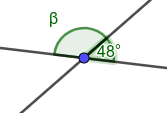
\includegraphics[width=2in]{geom-test1-review-img1.png}
\item Given the image below, and $m\angle BAC = 21^o$ and $m\angle BAD = 73^o$ find $m\angle CAD$.
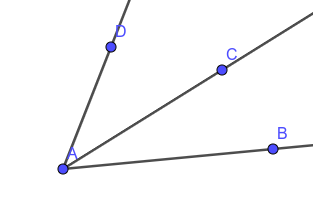
\includegraphics[width=2in]{geom-test1-review-img2.png}
\item What is the difference between $m\angle ABC$ and $\angle ABC$?
\end{enumerate}
\end{multicols}
\end{document}